%%\subsection{Webservers}

%%---------------------------------------------------------------------- 
\subsection{Apache}

\subsubsection{Tested with Versions} 
\begin{itemize}
\item Apache 2.4.6 linked against OpenSSL 1.0.1e, Debian jessie
\end{itemize}


\subsubsection{Settings} 

Enabled modules \emph{SSL} and \emph{Headers} are required.

%-All +TLSv1.1 +TLSv1.2
\begin{lstlisting}[breaklines]
  SSLCertificateFile server.crt
  SSLCertificateKeyFile server.key
  SSLProtocol All -SSLv2 -SSLv3 
  SSLHonorCipherOrder On
  SSLCompression off
  # Add six earth month HSTS header for all users...
  Header add Strict-Transport-Security "max-age=15768000"
  # If you want to protect all subdomains, use the following header
  # ALL subdomains HAVE TO support https if you use this!
  # Strict-Transport-Security: max-age=15768000 ; includeSubDomains

  SSLCipherSuite '@@@CIPHERSTRINGB@@@'

\end{lstlisting}

Note that any cipher suite starting with EECDH can be omitted, if in doubt.
(Compared to the theory section, EECDH in Apache and ECDHE in OpenSSL are
synonyms~\footnote{https://www.mail-archive.com/openssl-dev@openssl.org/msg33405.html})

\subsubsection{Additional settings}

You might want to redirect everything to http\textbf{s}:// if possible. In Apache you can do this with the following setting inside of a VirtualHost environment:

\begin{lstlisting}[breaklines]
  <VirtualHost *:80>
   #...
   RewriteEngine On
        RewriteRule ^.*$ https://%{SERVER_NAME}%{REQUEST_URI} [L,R=permanent]
   #...
  </VirtualHost>
\end{lstlisting}

%\subsubsection{Justification for special settings (if needed)}

\subsubsection{References}
\url{https://httpd.apache.org/docs/2.4/ssl/}


\subsubsection{How to test}

See appendix \ref{cha:tools}

%%\end{description}


%%---------------------------------------------------------------------- 
\subsection{lighttpd}



%%\begin{description}
\subsubsection{Tested with Version}
\begin{itemize}
\item lighttpd/1.4.31-4 with OpenSSL 1.0.1e on Debian 7.0
\item lighttpd/1.4.33 with OpenSSL 0.9.8o on Debian Squeeze (note that TLSv1.2 does not work in openssl 0.9.8 thus not all ciphers actually work)
\item lighttpd/1.4.28-2 with OpenSSL 0.9.8o on Debian Squeeze (note that TLSv1.2 does not work in openssl 0.9.8 thus not all ciphers actually work)
\end{itemize}


\subsubsection{Settings}


%% Complete ssl.cipher-list with same algo than Apache
\todo{FIXME: this string seems to be wrongly formatted??}

\begin{lstlisting}[breaklines]
  $SERVER["socket"] == "0.0.0.0:443" {
    ssl.engine  = "enable"
    ssl.use-sslv2 = "disable"
    ssl.use-sslv3 = "disable"
    #ssl.use-compression obsolete >= 1.4.3.1
    ssl.pemfile = "/etc/lighttpd/server.pem"
    ssl.cipher-list = "@@@CIPHERSTRINGB@@@"
    ssl.honor-cipher-order = "enable"
    setenv.add-response-header  = ( "Strict-Transport-Security" => "max-age=31536000")
  }
\end{lstlisting}


\subsubsection{Additional settings}

As for any other webserver, you might want to automatically redirect http
traffic toward http\textbf{s}:// It is also recommended to set the environment variable
\emph{HTTPS}, so the applications run by the webserver can easily detect, that
HTTPS is in use.



\begin{lstlisting}[breaklines]
  $HTTP["scheme"] == "http" {
    # capture vhost name with regex conditiona -> %0 in redirect pattern
    # must be the most inner block to the redirect rule
    $HTTP["host"] =~ ".*" {
        url.redirect = (".*" => "https://%0$0")
    }
  # Set the environment variable properly
  setenv.add-environment = (
            "HTTPS" => "on"
        )
  }
\end{lstlisting}


\subsubsection{Additional information} 
The config option \emph{honor-cipher-order} is available since 1.4.30, the
supported ciphers depend on the used OpenSSL-version (at runtime). ECDH has to
be available in OpenSSL at compile-time, which should be default. SSL
compression should by deactivated by default at compile-time (if not, it's
active).

Support for other SSL-libraries like GnuTLS will be available in the upcoming
2.x branch, which is currently under development.


\subsubsection{References} 

\begin{itemize}
        \item HTTPS redirection: \url{http://redmine.lighttpd.net/projects/1/wiki/HowToRedirectHttpToHttps}
        \item Lighttpd Docs SSL: \url{http://redmine.lighttpd.net/projects/lighttpd/wiki/Docs\_SSL}
        \item Release 1.4.30 (How to mitigate BEAST attack) \url{http://redmine.lighttpd.net/projects/lighttpd/wiki/Release-1\_4\_30}
        \item SSL Compression disabled by default: \url{http://redmine.lighttpd.net/issues/2445}
\end{itemize}




\subsubsection{How to test} 
See appendix \ref{cha:tools}



%%---------------------------------------------------------------------- 
\subsection{nginx}

%\begin{description}
\subsubsection{Tested with Version} 
\begin{itemize}
\item 1.4.4 with OpenSSL 1.0.1e on OS X Server 10.8.5
\item 1.2.1-2.2+wheezy2 with OpenSSL 1.0.1e on Debian 7.0
\item 1.4.4 with OpenSSL 1.0.1e on Debian 7.0
\item 1.2.1-2.2~bpo60+2 with OpenSSL 0.9.8o on Debian Squeeze (note that TLSv1.2 does not work in openssl 0.9.8 thus not all ciphers actually work)
\end{itemize}


\subsubsection{Settings}

\begin{lstlisting}[breaklines]
  ssl_prefer_server_ciphers on;
  ssl_protocols TLSv1 TLSv1.1 TLSv1.2; # not possible to do exclusive
  ssl_ciphers '@@@CIPHERSTRINGB@@@';
  add_header Strict-Transport-Security max-age=2592000;
\end{lstlisting}

If you absolutely want to specify your own DH parameters, you can specify them via

\begin{lstlisting}[breaklines]
  ssl_dhparam file;
\end{lstlisting}

However, we advise you to read section \ref{section:DH} and stay with the standard IKE/IETF parameters (as long as they are $ > 1024 $ bits).

\subsubsection{Additional settings}

If you decide to trust NIST's ECC curve recommendation, you can add the following line to nginx's configuration file to select special curves:

\begin{lstlisting}[breaklines]
  ssl_ecdh_curve          secp384r1;
\end{lstlisting}

You might want to redirect everything to http\textbf{s}:// if possible. In Nginx you can do this with the following setting:

\begin{lstlisting}[breaklines]
  return 301 https://$host$request_uri;
\end{lstlisting}


\subsubsection{References} 
\begin{itemize}
\item \url{http://nginx.org/en/docs/http/ngx_http_ssl_module.html}
\item \url{http://wiki.nginx.org/HttpSslModule}
\end{itemize}

\subsubsection{How to test}
See appendix \ref{cha:tools}





%%---------------------------------------------------------------------- 
\subsection{MS IIS}
\label{sec:ms-iis}

To configure SSL/TLS on Windows Server you can use IIS Crypto~\footnote{\url{https://www.nartac.com/Products/IISCrypto/}}
Simply start the Programm no installation required. The tool changes the registry keys described below.
A restart ist required for the changes to take effect.

\begin{figure}[p]
  \centering
  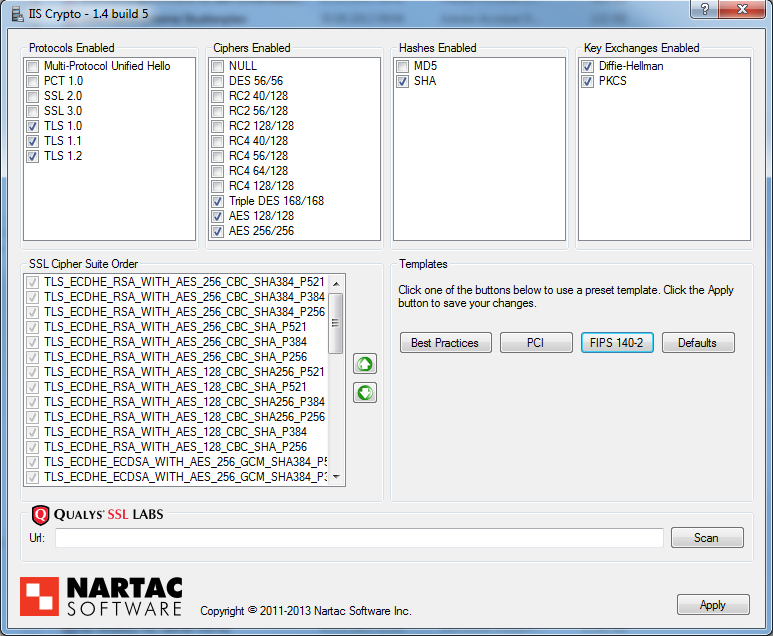
\includegraphics[width=0.411\textwidth]{img/IISCryptoFIPS1402.png}
  \caption{IIS Crypto Tool}
  \label{fig:IISCryptoFIPS1402}
\end{figure}

Instead of using the IIS Crypto Tool the configuration can be set
using the Windows Registry. The following Registry keys apply to the
newer Versions of Windows (Windows 7, Windows Server 2008, Windows
Server 2008 R2, Windows Server 2012 and Windows Server 2012 R2). For detailed
information about the older versions see the Microsoft knowlagebase
article. \footnote{\url{http://support.microsoft.com/kb/245030/en-us}}
\begin{lstlisting}[breaklines]
  [HKEY_LOCAL_MACHINE\SYSTEM\CurrentControlSet\Control\SecurityProviders\Schannel] 
  [HKEY_LOCAL_MACHINE\SYSTEM\CurrentControlSet\Control\SecurityProviders\Schannel\Ciphers] 
  [HKEY_LOCAL_MACHINE\SYSTEM\CurrentControlSet\Control\SecurityProviders\Schannel\CipherSuites] 
  [HKEY_LOCAL_MACHINE\SYSTEM\CurrentControlSet\Control\SecurityProviders\Schannel\Hashes] 
  [HKEY_LOCAL_MACHINE\SYSTEM\CurrentControlSet\Control\SecurityProviders\Schannel\KeyExchangeAlgorithms] 
  [HKEY_LOCAL_MACHINE\SYSTEM\CurrentControlSet\Control\SecurityProviders\Schannel\Protocols] 
\end{lstlisting}

Windows Server 2008 and Windows XP supports the following protocols:
\begin{itemize}
\item SSL 2.0
\item SSL 3.0
\item TLS 1.0
\end{itemize}

Windows Server 2008 R2 and newer and Windows 7 and newer support the following protocols:
\begin{itemize}
\item SSL 2.0
\item SSL 3.0
\item TLS 1.0
\item TLS 1.1
\item TLS 1.2
\end{itemize}

The srandard chipher order for TLS1.0 of Windows Server 2003 and Windows XP \footnote{\url{http://msdn.microsoft.com/en-us/library/windows/desktop/aa380512(v=vs.85).aspx}}
\begin{itemize}
\item TLS_RSA_WITH_RC4_128_MD5
\item TLS_RSA_WITH_RC4_128_SHA
\item TLS_RSA_WITH_3DES_EDE_CBC_SHA
\item TLS_DHE_DSS_WITH_3DES_EDE_CBC_SHA
\item TLS_RSA_WITH_DES_CBC_SHA
\item TLS_DHE_DSS_WITH_DES_CBC_SHA
\item TLS_RSA_EXPORT1024_WITH_RC4_56_SHA
\item TLS_RSA_EXPORT1024_WITH_DES_CBC_SHA
\item TLS_DHE_DSS_EXPORT1024_WITH_DES_CBC_SHA
\item TLS_RSA_EXPORT_WITH_RC4_40_MD5
\item TLS_RSA_EXPORT_WITH_RC2_CBC_40_MD5
\item TLS_RSA_WITH_NULL_MD5
\item TLS_RSA_WITH_NULL_SHA
\end{itemize}

the standard chipher order for Windows schannel.dll \footnote{\url{http://msdn.microsoft.com/en-us/library/windows/desktop/aa374757(v=vs.85).aspx}}
%%% i think this is for Windows Server 2008 R2 ab above. i will confirm in the near future.
\begin{table}[h]
  \centering
  \small
  \begin{tabular}{ll}
    \toprule
    Cipher suite	FIPS mode enabled	Exchange	Encryption	Hash	Protocols\\
    \midrule
\verb |TLS_RSA_WITH_AES_128_CBC_SHA256|Yes|TLS 1.2|RSA|AES|SHA256\\
\verb |TLS_RSA_WITH_AES_128_CBC_SHA|Yes|TLS 1.2, TLS 1.1, TLS 1.0|RSA|AES|SHA1\\
\verb |TLS_RSA_WITH_AES_256_CBC_SHA256|Yes|TLS 1.2|RSA|AES|SHA256\\
\verb |TLS_RSA_WITH_AES_256_CBC_SHA|Yes|TLS 1.2, TLS 1.1, TLS 1.0|RSA|AES|SHA1\\
\verb |TLS_RSA_WITH_RC4_128_SHA|No|TLS 1.2, TLS 1.1, TLS 1.0, SSL 3.0|RSA|RC4|SHA1\\
\verb |TLS_RSA_WITH_3DES_EDE_CBC_SHA|Yes|TLS 1.2, TLS 1.1, TLS 1.0|RSA|3DES|SHA1\\
\verb |TLS_ECDHE_RSA_WITH_AES_128_CBC_SHA256_P256|Yes|TLS 1.2|ECDH_P256|AES|SHA256\\
\verb |TLS_ECDHE_RSA_WITH_AES_128_CBC_SHA256_P384|Yes|TLS 1.2|ECDH_P384|AES|SHA256\\
\verb |TLS_ECDHE_RSA_WITH_AES_128_CBC_SHA_P256|Yes|TLS 1.2, TLS 1.1, TLS 1.0|ECDH_P256|AES|SHA1\\
\verb |TLS_ECDHE_RSA_WITH_AES_128_CBC_SHA_P384|Yes|TLS 1.2, TLS 1.1, TLS 1.0|ECDH_P384|AES|SHA1\\
\verb |TLS_ECDHE_RSA_WITH_AES_256_CBC_SHA_P256|Yes|TLS 1.2, TLS 1.1, TLS 1.0|ECDH_P256|AES|SHA1\\
\verb |TLS_ECDHE_RSA_WITH_AES_256_CBC_SHA_P384|Yes|TLS 1.2, TLS 1.1, TLS 1.0|ECDH_P384|AES|SHA1\\
\verb |TLS_ECDHE_ECDSA_WITH_AES_128_GCM_SHA256_P256|Yes|TLS 1.2|ECDH_P256|AES|SHA256\\
\verb |TLS_ECDHE_ECDSA_WITH_AES_256_GCM_SHA384_P384|Yes|TLS 1.2|ECDH_P384|AES|SHA384\\
\verb |TLS_ECDHE_ECDSA_WITH_AES_128_CBC_SHA256_P256|Yes|TLS 1.2|ECDH_P256|AES|SHA256\\
\verb |TLS_ECDHE_ECDSA_WITH_AES_128_CBC_SHA_P256|Yes|TLS 1.2, TLS 1.1, TLS 1.0|ECDH_P256|AES|SHA1\\
\verb |TLS_ECDHE_ECDSA_WITH_AES_128_CBC_SHA_P384|Yes|TLS 1.2, TLS 1.1, TLS 1.0|ECDH_P384|AES|SHA1\\
\verb |TLS_ECDHE_ECDSA_WITH_AES_256_CBC_SHA_P256|Yes|TLS 1.2, TLS 1.1, TLS 1.0|ECDH_P256|AES|SHA1\\
\verb |TLS_ECDHE_ECDSA_WITH_AES_256_CBC_SHA_P384|Yes|TLS 1.2, TLS 1.1, TLS 1.0|AES|SHA1\\
\verb |TLS_ECDHE_ECDSA_WITH_AES_256_CBC_SHA384_P384|Yes|TLS 1.2|ECDH_P384|AES|SHA384\\
\verb |TLS_DHE_DSS_WITH_AES_128_CBC_SHA256|Yes|TLS 1.2|DH|AES|SHA256v
\verb |TLS_DHE_DSS_WITH_AES_128_CBC_SHA|Yes|TLS 1.2, TLS 1.1, TLS 1.0|DH|AES|SHA1\\
\verb |TLS_DHE_DSS_WITH_AES_256_CBC_SHA256|Yes|TLS 1.2|DH|AES|SHA256\\
\verb |TLS_DHE_DSS_WITH_AES_256_CBC_SHA|Yes|TLS 1.2, TLS 1.1, TLS 1.0|DH|AES|SHA1\\
\verb |TLS_DHE_DSS_WITH_3DES_EDE_CBC_SHA|Yes|TLS 1.2, TLS 1.1, TLS 1.0, SSL 3.0|DH|3DES|SHA1\\
\verb |TLS_RSA_WITH_RC4_128_MD5|No|TLS 1.2, TLS 1.1, TLS 1.0, SSL 3.0|RSA|RC4|MD5\\
\verb |SSL_CK_RC4_128_WITH_MD5|No|SSL 2.0|RSA|RC4|MD5\\
\verb |SSL_CK_DES_192_EDE3_CBC_WITH_MD5|No|SSL 2.0|RSA|3DES|MD5\\
\verb |TLS_RSA_WITH_NULL_SHA256|No|TLS 1.2|RSA|NULL|SHA256\\
\verb |TLS_RSA_WITH_NULL_SHA|No|TLS 1.2, TLS 1.1, TLS 1.0, SSL 3.0|RSA|NULL|SHA1\\
 \bottomrule 
 \end{tabular}
  \caption{Client support}
  \label{tab:MS_IIS_Client_Support}
\end{table}
Note that the the following cipher suites are supported, but they are not enabled by default.
They must be added as necessary. 

\begin{itemize}
\item TLS_RSA_EXPORT_WITH_RC4_40_MD5
\item TLS_RSA_EXPORT1024_WITH_RC4_56_SHA
\item TLS_RSA_EXPORT1024_WITH_DES_CBC_SHA
\item SSL_CK_RC4_128_EXPORT40_MD5
\item SSL_CK_DES_64_CBC_WITH_MD5
\item TLS_RSA_WITH_DES_CBC_SHA
\item TLS_RSA_WITH_NULL_MD5
\item TLS_RSA_WITH_NULL_SHA
\item TLS_DHE_DSS_EXPORT1024_WITH_DES_CBC_SHA
\item TLS_DHE_DSS_WITH_DES_CBC_SHA
\item TLS_ECDHE_ECDSA_WITH_AES_128_CBC_SHA_P521
\item TLS_ECDHE_ECDSA_WITH_AES_256_CBC_SHA_P521
\item TLS_ECDHE_ECDSA_WITH_AES_128_CBC_SHA256_P384
\item TLS_ECDHE_ECDSA_WITH_AES_128_CBC_SHA256_P521
\item TLS_ECDHE_ECDSA_WITH_AES_256_CBC_SHA384_P521
\item TLS_ECDHE_ECDSA_WITH_AES_128_GCM_SHA256_P384
\item TLS_ECDHE_ECDSA_WITH_AES_128_GCM_SHA256_P521
\item TLS_ECDHE_ECDSA_WITH_AES_256_GCM_SHA384_P521
\item TLS_ECDHE_ECDSA_WITH_AES_128_GCM_SHA256_P384
\item TLS_ECDHE_RSA_WITH_AES_128_CBC_SHA_P521
\item TLS_ECDHE_RSA_WITH_AES_256_CBC_SHA_P521
\item TLS_ECDHE_RSA_WITH_AES_128_CBC_SHA256_P521
\item TLS_ECDHE_RSA_WITH_AES_256_CBC_SHA384_P256
\item TLS_ECDHE_RSA_WITH_AES_256_CBC_SHA384_P384
\item TLS_ECDHE_RSA_WITH_AES_256_CBC_SHA384_P521
\end{itemize}

%\begin{description}

\subsubsection{Tested with Version} \todo{Daniel: add tested version}

\begin{itemize}
\item Windows Server 2012 R2 and Windows 8.1 using IE11 and Chrome 31
\item Windows Server 2012 R2 and MacOS 10.9.1 using Safari 7 and Chrome 31
%%% I used the FIPS 140 configuration of IIS Crypto. Should i test this with the standard configuration a & b?
%%% I can test this down to windows 7 an Server 2008 ... Windows XP ist no longer supported by Microsoft so i dont care.
\end{itemize}

\subsubsection{Settings}


When trying to avoid RC4 and CBC (BEAST-Attack) and requiring perfect
forward secrecy, Microsoft Internet Information Server (IIS) supports
ECDSA, but does not support RSA for key exchange (consider ECC suite
B doubts\footnote{\url{http://safecurves.cr.yp.to/rigid.html}}).

Since \verb|ECDHE_RSA_*| is not supported, a SSL certificate based on
elliptic curves needs to be used.

The configuration of cipher suites MS IIS will use, can be configured in one
of the following ways:
\begin{enumerate}
\item Group Policy \footnote{\url{http://msdn.microsoft.com/en-us/library/windows/desktop/bb870930(v=vs.85).aspx}}
\item Registry \footnote{\url{http://support.microsoft.com/kb/245030/en-us}}
\item IIS Crypto~\footnote{\url{https://www.nartac.com/Products/IISCrypto/}}
\end{enumerate}


Table~\ref{tab:MS_IIS_Client_Support} shows the process of turning on
one algorithm after another and the effect on the supported clients
tested using https://www.ssllabs.com.

\verb|SSL 3.0|, \verb|SSL 2.0| and \verb|MD5| are turned off.
\verb|TLS 1.0| and \verb|TLS 2.0| are turned on.
%%% Lets use the common name for TLS 1.2

\begin{table}[h]
  \centering
  \small
  \begin{tabular}{ll}
    \toprule
    Cipher Suite & Client \\
    \midrule
    \verb|TLS_ECDHE_ECDSA_WITH_AES_128_GCM_SHA256| & only IE 10,11, OpenSSL 1.0.1e \\
    \verb|TLS_ECDHE_ECDSA_WITH_AES_128_CBC_SHA256| & Chrome 30, Opera 17, Safari 6+ \\
    \verb|TLS_ECDHE_ECDSA_WITH_AES_128_CBC_SHA| & FF 10-24, IE 8+, Safari 5, Java 7\\
    \bottomrule 
 \end{tabular}
  \caption{Client support}
  \label{tab:MS_IIS_Client_Support}
\end{table}

Table~\ref{tab:MS_IIS_Client_Support} shows the algorithms from
strongest to weakest and why they need to be added in this order. For
example insisting on SHA-2 algorithms (only first two lines) would
eliminate all versions of Firefox, so the last line is needed to
support this browser, but should be placed at the bottom, so capable
browsers will choose the stronger SHA-2 algorithms.

\verb|TLS_RSA_WITH_RC4_128_SHA| or equivalent should also be added if
MS Terminal Server Connection is used (make sure to use this only in a
trusted environment). This suite will not be used for SSL, since we do
not use a RSA Key.


% \verb|TLS_ECDHE_ECDSA_WITH_AES_128_GCM_SHA256| ... only supported by: IE 10,11, OpenSSL 1.0.1e
% \verb|TLS_ECDHE_ECDSA_WITH_AES_128_CBC_SHA256| ... Chrome 30, Opera 17, Safari 6+
% \verb|TLS_ECDHE_ECDSA_WITH_AES_128_CBC_SHA| ... Firefox 10-24, IE 8+, Safari 5, Java 7


Clients not supported:
\begin{enumerate}
\item Java 6
\item WinXP
\item Bing
\end{enumerate}

\subsubsection{Additional settings}

%Here you can add additional settings
You might want to redirect everything to http\textbf{s}:// if possible. In IIS you can do this with the following setting by Powershell:

\begin{lstlisting}[breaklines]
Set-WebConfiguration -Location "$WebSiteName/$WebApplicationName" `
    -Filter 'system.webserver/security/access' `
    -Value "SslRequireCert"
\end{lstlisting}

or using the GUI as shown in figure XXX
\todo add screenshot here



\subsubsection{Justification for special settings (if needed)}

% in case you have the need for further justifications why you chose this and that setting or if the settings do not fit into the standard Variant A or Variant B schema, please document this here

\subsubsection{References}

\todo{add references}

\begin{itemize}
\item \url{http://support.microsoft.com/kb/245030/en-us}
\item \url{http://support.microsoft.com/kb/187498/en-us}
\end{itemize}

% add any further references or best practice documents here

\subsubsection{How to test}
See appendix \ref{cha:tools}


%\end{description}

%%% Local Variables: 
%%% mode: latex
%%% TeX-master: "../applied-crypto-hardening"
%%% End: 
